\chapter{Java Virtual Machine Tool Interface (JVMTI)}
\section{Introduction} % 1/2
Before this work started the basic approach of debugging java code that runs in the CACAO virtual machine was either to enable the command line option \textit{verbose:call}, use gdb or insert debug statements in the java code itself. Debugging java code this way can be a very tedious job. Therefore this work was started with the aim to give developers a better support for debugging java code that runs in the CACAO java virtual machine.

Other projects had already started similar efforts like SableVM\cite{sablevm} and Redhat in GIJ\cite{gij}. To take advantage of the numerous already existing Java debugging front-ends both project implemented Sun's Java Debug Wire Protocol (JDWP)\cite{jpda}. Whereas the JDWP implementation in SableVM is older and tight coupled with the virtual machine itself, Redhat's implementation been committed to the GNU classpath project and is expected to be integrated in other virtual machines. For this reason the decision has been taken to implement JVMTI\cite{jvmti} as being the lowest layer of the Java Platform Debugger Architecture(JPDA)\cite{jpda}.

\section{The Sun Java Platform Debugger Architecture (JPDA)} % 2
Throughout this document I will refer to the version of the Java Platform Debugger Architecture\cite{jpda} introduced by Sun Microsystems with Java 2 Standard Edition (J2SE) 5.0.

\subsection{Architecture} % 1
As it is sketched out in figure \ref{fig:jdpa} the JPDA is composed by three layers. The highest layer is the Java Debug Interface (JDI) which defines a high level interface which was developed for debugger developers to write remote debuggers easily. 

JDI itself is built on top of JDWP. The Java Debug Wire Protocol (JDWP) represents the communication layer between the debugger and the debuggee process. 

The lowest layer in the JPDA is the Java Virtual Machine Tool Interface (JVMTI) which is used by the JDWP back-end to interact with the virtual machine. JVMTI was introduced in J2SE 5.0 and replaced the Java Virtual Machine Debug Interface (JVMDI).

\begin{figure}[h]
	\centering
	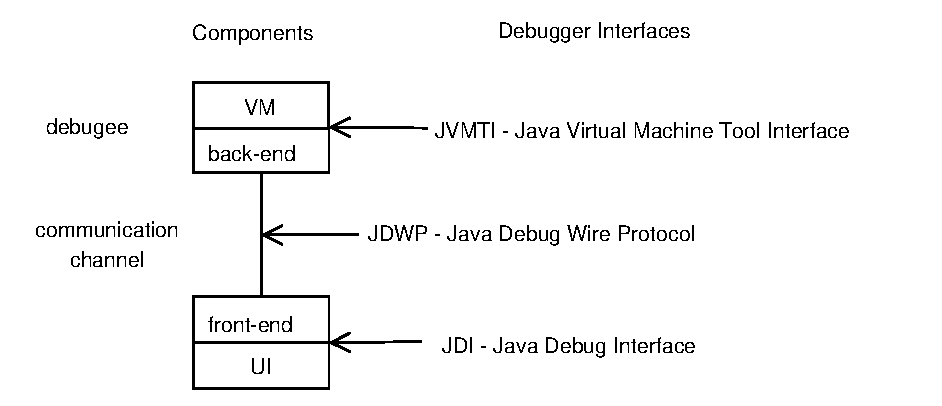
\includegraphics[scale=.75]{arch.eps}
	\caption{Java Platform Debugger Architecture overview\cite{jpda}}
	\label{fig:jdpa}
\end{figure}


According to the JPDA specification a debugger may be built on top of any of this three layers depending on their need of lower level functionalities.


\subsection{Java Virtual Machine Tool Interface (JVMTI)} % 1-2
JVMTI is two-way interface that enables its client to get information about the state of the virtual machine and the java program that is being executed or alter it. The client can also set callback function to be informed about the occurrence of specified events.

\subsubsection{Invoking JVMTI}
JVMTI environments can be created either in a so called jvmti agent or in a java native method. Each JVMTI environment contains client defined callbacks, event notification modes, capabilities and a environment local storage. Similar to the JNI opaque pointer the JVMTI environment pointer is used to call JVMTI functions by dereferencing the JVMTI environment pointer twice.

A jvmti agent is a shared library that contains a \textit{Agent\_OnLoad} function that is called on startup by the virtual machine. In the \textit{Agent\_OnLoad} function an agent is only allowed to call jvmti functions because other parts of the virtual machine are not yet initialized. On shut down the the virtual machine calls \textit{Agent\_UnLoad} to allow the agent to shut down gracefully. The user can specify the jvmti agent by using either the argument \textit{agentlib} or \textit{agentpath}.

\begin{figure}[h]
\begin{verbatim}
          -agentlib:<agent-lib-name>=<options>
          -agentpath:<path-to-agent>=<options>
\end{verbatim}
\caption{Command line arguments to load a JVMTI agent}
\end{figure}

The opaque pointer to a new JVMTI environment can be obtained through the Java Invocation API by calling GetEnv.

\begin{figure}[h]
\begin{verbatim}
  (*javavm)->
       GetEnv(javavm, &jvmti_environment, JVMTI_VERSION_1_0)
\end{verbatim}
\caption{Java Invocation API call to get a new JVMTI environment}
\end{figure}

This can be done in a Java native method or in the AgentOnLoad function.

\subsubsection{Functions}
\label{jvmtifunctions}
JVMTI functions get called by dereferencing the JVMTI environment pointer twice. Every JVMTI function has jvmtiError as its return type. As you can see in figure \ref{functioncall} the result of a function call is stored in an variable pointed to by an other parameter to the function call.

\begin{figure}[h]
\begin{verbatim}
  jint version;
  ...
  jvmtiError error = 
     (*jvmti_environment)->
          GetVersionNumber(jvmti_environment, &version);
\end{verbatim}
\caption{Example JVMTI function call to GetVersionNumber.}
\label{functioncall}
\end{figure}

The java virtual machine tool interface defines 120 required and optional functions. Their functionality ranges from thread, thread group, stack frame, local variable, heap, class, field, method and system properties inspection and manipulation to setting breakpoints, watch fields or timers. Additionally there are function to support writing JVMTI agents and JVMTI management functions. For a detailed description of the single functions please refer to the JVMTI specification\cite{jvmti}.

The functions that can be called within a particular environment are restricted by the phase in which the virtual machine is currently running and the capabilities that a given JVMTI environment has obtained by the virtual machine.

JVMTI defines the phase \textit{onload}, \textit{primordial}, \textit{start}, \textit{live} and \textit{dead}. The \textit{onload} phase takes just as long as the AgentOnLoad function is running. Between the \textit{onload} and the \textit{start} phase there is the \textit{primordial} phase. In this phase only some jvmti functions can be called and JNI is not live yet. From \textit{start} phase on JNI calls are allowed but the virtual machine is not yet fully initialized. In the \textit{live} phase the java virtual machine is fully initialized. The final phase is \textit{dead}, which is active during the termination of the virtual machine.

The java virtual machine tool interface has required and optional functions. The capabilities of a JVMTI environment show what optional function may be called by a given environment. A new environment has no optional capabilities enabled. Therefore to call optional functions the function \textit{Add Capabilities} has to be called first. To get all available capabilities a call to \textit{Get Potential Capabilities} is needed.


\subsubsection{Events}
JVMTI defines 30 events that can occur on a breakpoint hit, single step, class or method state change, exceptions, phase change, garbages collections, method invocation, monitor enter, field access, thread start or end. For a detailed description of the single events please refer to the JVMTI specification\cite{jvmti}.

As for JVMTI functions, events are influenced by the phase the virtual machine is in and the capabilities of the JVMTI environment. To be able to handle events a JVMTI agent needs to set callback function that will be executed by the virtual machine on occurrence of the event. This is done by calling \textit{Set Event Callbacks}. After setting event callbacks, events have to be enabled by calling \textit{Set Event Notification Mode}. This function may return an error if the capability for a given event is not available in the current JVMTI environment.

\section{GNU classpath JDWP} % 2
GNU classpath JDWP is almost a complete implementation of Sun's JDWP specification. The drawback is that it was not build with JVMTI in mind. Therefore a few adaptions were needed to make it work with JVMTI and CACAO.

\subsection{Invocation} % 1/2
Because CACAO should work with existing Java debugging front-ends, like eclipse\cite{eclipse}, it was chosen to make the command line arguments compatible with Sun's JDK. Therefore JDWP can be started in CACAO by using either the \textit{-agentlib}, \textit{-agentpath} or the old \textit{-Xdebug} and \textit{-Xrunjdwp} arguments. 

\begin{figure}[h]
\begin{verbatim}

                  cacao -agentlib:jdwp=help
\end{verbatim}
\caption{Invocation of cacao jdwp help}
\end{figure}

The invocation of GNU classpath JDWP itself is the same for both kind of arguments. On start-up of CACAO, immediately after all command line arguments for the virtual machine have been processed, the JVMTI agent libjdwp.so is called.

In its Agent\_OnLoad function all JDWP related options are processed, a new JVMTI environment is created, all JDWP relevant callbacks are set, all capabilities are added and the \textit{VM\_INIT} event is enabled. 

The \textit{VM\_INIT} event is triggered after the virtual machine has been fully initialized and before the main class is executed. In the callback a new GNU classpath JDWP object is created and the JDWP listening thread is started. This permits the user to take control of the execution of the java program before it effectively starts.

\subsection{JDWP-JVMTI interface} % 1 /2
After the JDWP listening thread has been started, every communication between GNU classpath JDWP and CACAO JVMTI takes place through the JDWP-JVMTI glue code. It consists of the implementation of all java native methods in the VMVirtualMachine, VMMethod and VMFrame classes of the gnu.classpath.jdwp package and the callback functions in VMJdwp.

The GNU classpath JDWP native methods contain all virtual machine dependent functions that JDWP needs. Because CACAO supports JVMTI those native methods are implemented using different JVMTI function calls.

To facilitate the delivery of JVMTI events to the JDWP layer, new \texttt{gnu.classpath.jdwp.event}-objects are created. Each event type is enclosed in its own event class.  Each of those event objects represent a single event which is sent by calling the static java method \texttt{Jdwp.notify(event ev)}. This is done within each JVMTI callback function using JNI function calls.



\section{JVMTI implementation in CACAO} % 5

The main goals that led the development of JVMTI in CACAO were to enable developers to debug their software efficiently and minimize the influence and interference of JVMTI code on the normal runtime behaviour of the CACAO virtual machine.

\subsection{Architecture} % 1

The architectural decisions for the JVMTI implementation in CACAO were mainly complicated by the fact that CACAO uses a just in time compiler to execute java code. Due to that, key functionality, like \textit{breakpoint} and \textit{single step} events, need \textit{ptrace}\cite{ptrace} support.

The easiest way to implement other JVMTI events would be to compile direct function calls for firing jvmti events in the normal CACAO code. This approach is used to implement events that are supposed to happen rarely, like thread-start/end or phase change events.

If this approach would be used on events that occur very often, like \textit{Method Enter} and \textit{Method Exit}, the runtime behaviour would be strongly influenced by a significant slow down of the virtual machine. The fact that JVMTI can be started and stopped multiple times during the lifetime of the virtual machine, makes this problem even worse because of that the event firing code needs to be always compiled in and therefore slowing down the virtual machine even in situations where no debugging facility is needed.

\subsubsection{Debugging support processes}
As mentioned earlier the CACAO JVMTI implementation needs \textit{ptrace} to implement breakpoints and other events. Due to that a parent (debugger) process, that handles traps (\texttt{SIGTRAP}) and other signals, is needed. 

Such a debugger process needs to be aware of many operating system, library and processor specifics. Because of that, and due to the fact that CACAO runs on several different processor, library and operating system configurations, the decision has been taken to use GNU debugger\cite{gdb} (\textit{gdb}) as debugger process and control gdb with a third process (\textit{cacaodbgserver}).

\begin{figure}[h]
\begin{verbatim}
                cacao 
                   \_  -cacaodbgserver
                            \_  -gdb
\end{verbatim}
\caption{Process structure of a running JVMTI session}
\label{processstructure}
\end{figure}


The gdb and its control process are lunched by need during the creation of a new JVMTI environment and are killed after the last JVMTI environment gets disposed.

\subsubsection{Event handling with traps}
\label{eventhandling}
Gdb normally implements breakpoints by using so called trap instructions. These instructions (e.g. \texttt{int3} on i386) are put in the place where the breakpoint has to be fired. On execution of a trap instruction the operating system sends a \texttt{SIGTRAP} signal to the tracing process. At that point the tracing process is able to inspect and change the traced process.

Setting trap instructions in CACAO JVMTI is a major problem if a trap lays in JIT compiler generated code because there is the need for JIT compiler support to get the appropriate position where to put the trap. The second JIT compiler issue is related to the possibility of the JIT compiler to patch and recompile a method. Such patching or recompilation will overwrite existing trap instructions. The way CACAO deals with these issues is described in section \ref{traps}.

CACAO JVMTI has to execute the appropriate event callbacks if it gets a \texttt{SIGTRAP}. To accomplish this the controlling process \textit{cacaodbgserver} uses the gdb process to call \texttt{jvmti\_cacao\_generic\_breakpointhandler} from within the current execution thread of the cacao virtual machine. This function executes all enabled event callbacks, for this kind of event, in the current execution thread. It is important to note that during the execution of a callback the execution of other virtual machine java threads is not stopped. To explicitly stop other running threads the JVMTI function SuspendThread has to be called.

%call
% continuing thread execution

\subsubsection{JLocation format}
\label{jlocation}
JLocation is the return type of many JVMTI functions and events representing some java bytecode location in the virtual machine. Sun's JVMTI specification\cite{jvmti} leaves the JLocation type intentionally unconstrained. The greatest functionality is achieved with JLocation indicating the bytecode index of a java instruction, but virtual machines, like CACAO, that do not have an appropriate mapping to the bytecode indexing scheme are allowed to use the native program counter or some other representation. This format has to be ``A 64 bit value, representing a monotonically increasing executable position within a method. -1 indicates a native method.''\cite{jvmti}. 

% mapping - line number

\begin{table}[h]
\begin{center}
\begin{tabular}{|l|l|l|}
\hline
\multicolumn{3}{|c|}{Mapping to JLocation}\\\hline
function/event Name & support functionality & available \\\hline
\hline
Get Stack Trace  & stacktrace &line number \\\hline
Get Frame Location & stacktrace & line number\\\hline %  : return the location of the instruction currently executing
Get Line Number Table & line number table & line number \\\hline
Get Method Location &   line number table  & line number \\\hline
Breakpoint & stacktrace  & line number \\\hline
SingleStep & stacktrace  & line number \\\hline
Exception & stacktrace   & line number \\\hline
Exception Catch & stacktrace & line number \\\hline
Get Local Variable Table & local variable table and &\\
                                    & line number table & line number \\\hline
Field Access & stacktrace & line number \\\hline
Field Modification & stacktrace & line number \\\hline
Compiled Method Load & line number table & line number \\\hline
\hline
\multicolumn{3}{|c|}{Mapping from JLocation} \\\hline
\hline
function/event Name & support functionality & available \\\hline
Set Breakpoint & line number table   & line number\\\hline
Clear Breakpoint &  line number table  & line number \\\hline
\end{tabular}
\end{center}
\caption{Needed JLocation mapping}
\label{JLocationmapping}
\end{table} 

The decision has been taken to use a JLocation format other then bytecode index and native program counter. As you can see in table \ref{JLocationmapping} all JVMTI function and events could support line numbers as being the JLocation format in the CACAO virtual machine. Therefore line numbers will be used as JLocations. The second column (support functionality) of table \ref{JLocationmapping} specifies the functions and data structures that are needed to get a correct JLocation value.

\subsubsection{Enabling traps}
\label{traps}
As described in section \ref{eventhandling}, there are two major issues using traps in JIT compiler generated code. 

The first issue, concerning the mapping of a JLocation position to a native program counter position, can be dealt with by the JIT compiler, by filling in the line number table with current native program counter values. This is already done by the JIT compiler to support java stack traces. Furthermore the JIT compiler has to mark special positions like method enter/exit, exception throwing and exception catching. Figure \ref{scenariocompile} shows a high level pseudo code of how the JIT compiler can support JVMTI events.

\begin{figure}[h]
\begin{verbatim}

- compile method
- fill in line number table with native pc values
- if ((breakpoints or method enter or method exit or
      exception or exception catch) events are enabled) 
        call jvmti to set traps with current pc values
\end{verbatim}
\caption{Scenario: (re-)compile a method}
\label{scenariocompile}
\end{figure}


The second issue, about overwriting existing traps during a recompilation or patching of an already compiled method, can be dealt with by updating the line number table and special positions before resetting those traps. Figure \ref{scenariopatch} shows a high level pseudo code of how the CACO patcher can support JVMTI events.

\begin{figure}[h]
\begin{verbatim}

- patch method
- update line number table with native pc values
- if ((breakpoints or method enter or method exit or
      exception or exception catch) events are enabled) 
        call jvmti to reset traps with updated pc values
\end{verbatim}
\caption{Scenario: patch an already compiled method}
\label{scenariopatch}
\end{figure}

This approach moreover has the advantage to allow JVMTI to easily disable some or all traps if they are no more needed.

\subsection{Implemented Features} % 2
As described in section \ref{jvmtifunctions}, JVMTI has many optional funtcions and events. CACAO does not implement all optional JVMTI function and events yet. Table \ref{implementedfunctions} and \ref{implementedevents} show what functions and events CACAO JVMTI supports.

\begin{table} [h]
\begin{center}
\begin{tabular}{|l|l|}
\hline
Function category & Supported functions\\\hline\hline
Memory Management& all \\\hline
Thread& all \\\hline
Thread Group& all \\\hline
Stack Frame& Pop Frame and Notify Frame Pop missing \\\hline
Heap& only Force Garbage Collection \\\hline
Local Variables& none \\\hline
Breakpoint& all ? \\\hline
Watched Field& none \\\hline
Class& Get Source Debug Extension and \\
        &  Redefine Classes missing \\\hline
Object& GetObjectMonitorUsage missing \\\hline
Field& IsFieldSynthetic missing \\\hline
Method& Is Method Synthetic and \\
           & Is Method Obsolete missing \\\hline
Raw Monitor& all \\\hline
JNI Function Interception& all \\\hline
Event Management& Generate Events missing \\\hline
Extension Mechanism& cacao jvmti has no extended functions \\\hline
Capability& all \\\hline
Timers& Get Timer Information, Get Time \\\hline
System Properties& all \\\hline
General& all \\\hline
 \end{tabular}\end{center}
\caption{Supported JVMTI functions in CACAO}
\label{implementedfunctions}
\end{table} 


\begin{table} [h]
\begin{center}
\begin{tabular}{|l|c|}
\hline
Event groups & Supported\\\hline\hline
Breakpoint/Single Step & yes \\ % todo
Class File Load Hook/Load/Prepare  & yes \\ % to test
Compiled Method Load/Unload  & no\\
Data Dump Request  & yes \\
Dynamic Code Generated  & yes \\
Exception/Exception Catch  & yes \\
Field Access/Modification  & no \\
Frame Pop  & no \\
Garbage Collection Finish/Start  & no \\
Method Entry/Exit  & yes \\
Monitor Contended Enter/Entered  & yes \\
Monitor Wait/Waited  & yes \\
Native Method Bind  & yes \\
Object Free  & no \\
Thread Start/End  & yes \\
VM Start/Initialization/Death Event  & yes \\
VM Object Allocation  & no \\
\hline
\end{tabular}\end{center}
\caption{Supported JVMTI events in CACAO}
\label{implementedevents}
\end{table} 

\subsection{Further work}
As JVMTI is a huge interface not all functionality is already implemented in CACAO. To further ease debugging of Java programs, support of inspecting and changing local variables should be added. 

Beside debugging JVMTI is also meant to support profiling which is not supported at all in the current CACAO JVMTI implementation.


